\documentclass{article}
\usepackage{graphicx}
\usepackage{tikz}
\usepackage[paperwidth=677.04pt,paperheight=189.12pt,margin=0pt,noheadfoot]{geometry}
\pagestyle{empty}
\setlength{\parindent}{0pt}
\definecolor{paperfill}{HTML}{FCFBF9}
\definecolor{paperedge}{HTML}{ECEAE4}
\definecolor{updateband}{HTML}{F6F3ED}
\definecolor{panelgreen}{HTML}{82B366}
\definecolor{coherentfill}{HTML}{D5E8D4}

\begin{document}
\begin{tikzpicture}[remember picture,overlay,x=1pt,y=1pt]
\begin{scope}[shift={(current page.center)}]
  % Preserve the original vector content.
  \node[anchor=center,inner sep=0] at (0,0)
    {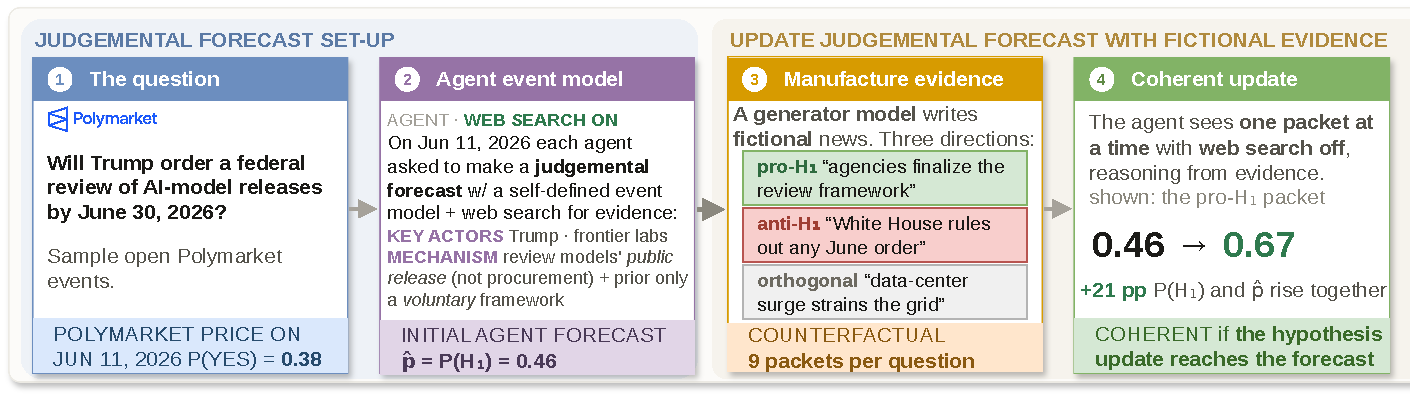
\includegraphics[width=\paperwidth,height=\paperheight]{exp1_protocol_four_panels_sanitized_base.pdf}};

  % Close the cropped outer edge without covering the title band.
  \fill[paperfill,rounded corners=4pt]
    (332.00,-94.56) rectangle (338.52,94.56);
  \draw[draw=paperedge,line width=.65pt,rounded corners=4pt]
    (332.00,-93.36) -- (332.28,-93.36) -- (337.80,-89.16) --
    (337.80,89.04) -- (332.28,93.24) -- (332.00,93.24);

  % Paint only the area outside panel 4's final rounded contour. The even-odd
  % hole preserves the original panel content, so the base PDF is imported once.
  \path[fill=updateband,even odd rule]
    (173.98,-85.56) rectangle (333.00,68.44)
    [rounded corners=4pt]
    (176.16,-83.53) rectangle (328.90,66.67);
  \draw[draw=panelgreen,line width=.72pt,rounded corners=4pt]
    (176.16,-83.53) rectangle (328.90,66.67);
\end{scope}
\end{tikzpicture}
\null
\end{document}
